\documentclass[tikz,border=5mm]{standalone}
\begin{document}
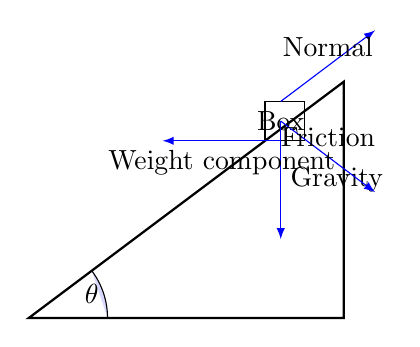
\begin{tikzpicture}[force/.style={>=latex,draw=blue,fill=blue}]

% Draw the inclined plane
\draw[thick] (0,0) -- (4,0) -- (4,3) -- cycle;

% Angle of inclination
\draw[fill=blue!15] (1,0) arc (0:37:1);
\node at (0.8,0.3) {$\theta$};

% Draw the box
\draw (3,2.25) rectangle ++(0.5, 0.5);
\node at (3.2,2.5) {Box};

% Draw and label forces
\draw[force,->] (3.2,2.5) --++ (0,-1.5) node[midway,right] {Gravity};
\draw[force,->] (3.2,2.75) --++ (37:1.5) node[midway,above] {Normal};
\draw[force,->] (3.2,2.5) --++ (-37:1.5) node[midway,above] {Friction};
\draw[force,->] (3.2,2.25) --++ (0:-1.5) node[midway,below] {Weight component};

\end{tikzpicture}
\end{document}

